\documentclass[conference]{IEEEtran}
\IEEEoverridecommandlockouts
\usepackage{cite}
\usepackage{amsmath,amssymb,amsfonts}
\usepackage{algorithmic}
\usepackage{graphicx}
\usepackage{textcomp}
\usepackage{xcolor}
\usepackage{iftex}

% Native Multilingual Font Support for Overleaf (XeLaTeX engine)
\ifXeTeX
  \usepackage{fontspec}
  \newfontfamily\hindifont{Noto Sans Devanagari}[Script=Devanagari]
  \newfontfamily\telugufont{Noto Sans Telugu}[Script=Telugu]
  \newfontfamily\bengalifont{Noto Sans Bengali}[Script=Bengali]
  \newcommand{\texthindi}[1]{{\hindifont #1}}
  \newcommand{\texttelugu}[1]{{\telugufont #1}}
  \newcommand{\textbengali}[1]{{\bengalifont #1}}
\else
  % Fallback definition if compiled under pdfLaTeX (prevents undefined macro errors)
  \newcommand{\texthindi}[1]{#1}
  \newcommand{\texttelugu}[1]{#1}
  \newcommand{\textbengali}[1]{#1}
\fi

\begin{document}

% ==================== TITLE & AUTHORS ====================
\title{IndicSQL: Schema-Grounded Multilingual Text-to-SQL for Indian Governance Open Data}

\author{
\IEEEauthorblockN{Author Names Anonymous for Peer Review}
\IEEEauthorblockA{\textit{Department of Computer Science and Engineering} \\
\textit{Autonomous Multi-Agent Systems Laboratory}\\
New Delhi, India \\
contact@indicsql-research.org}
}

\maketitle

% ==================== ABSTRACT ====================
\begin{abstract}
While Large Language Models have advanced Text-to-SQL semantic parsing on English benchmarks, non-Western administrative databases present severe cross-lingual grounding barriers. Benchmarks such as \textsc{IndicDBBench} document a persistent 9.0--12.8 percentage point performance drop (the ``Indic Gap'') between English and Indic queries across monolithic models. We present \textsc{IndicSQL}, an autonomous multi-agent Text-to-SQL architecture designed to resolve cross-lingual schema linking and structural query decomposition over complex Indian administrative databases. \textsc{IndicSQL} coordinates a five-agent collaborative pipeline for multilingual schema routing, metric planning, relational catalog grounding, execution validation, and native response verbalization. We establish a reproducible zero-shot baseline on the \textsc{IndicDBBench} PostgreSQL corpus evaluated across 280 sealed test instances spanning English, Hinglish, Hindi, Marathi, Bengali, Tamil, and Telugu under deterministic cryptographic locks. Using open-weights \textsc{Qwen-2.5-7B-Instruct}, \textsc{IndicSQL} achieves 98.9\% schema-routing accuracy (277/280), 54.6\% SQL execution success (153/280), and an overall 22.5\% execution match (EX, 63/280). In our parallel multilingual evaluation, native queries in Hindi, Hinglish, and Tamil (each 27.5\% EX) achieve an observed +10.0 percentage-point gain over the English baseline (17.5\% EX), suggesting that modular intent abstraction mitigates the subword token fertility penalty. A rigorous error audit of the 128 non-executable evaluations reveals that 96 cases (75.0\%) stem from column identifier hallucinations against deep relational schemas (chains to depth 6), 25 cases (19.5\%) from PostgreSQL runtime execution timeouts ($>60$\,s) induced by missing join predicates, and 7 cases (5.5\%) from upstream benchmark reference defects. Ablation experiments confirm that modular planning and schema routing improve EX by +13.6\,pp over monolithic prompting, framing a verifiable foundation for future domain-adapted fine-tuning.
\end{abstract}

\begin{IEEEkeywords}
Text-to-SQL, Natural Language Interfaces to Databases, Multi-Agent Systems, Semantic Parsing, Indic Languages, Schema Grounding, Response Verbalization.
\end{IEEEkeywords}

% ==================== SECTION I: INTRODUCTION ====================
\section{Introduction}\label{sec:intro}
Public open-government portals in India, such as the National Data and Analytics Platform (NDAP) and the India Data Portal (IDP), host invaluable relational datasets spanning healthcare delivery, demographics, and agriculture. However, unlocking these repositories for citizens and administrators through natural language query interfaces remains fundamentally difficult. Unlike curated English benchmarks such as Spider~\cite{yu2018spider} and BIRD~\cite{li2023bird}, Indian governance databases present high relational join depths (often requiring traversal across up to six intermediate tables) and rely on compressed, non-standard departmental abbreviations (e.g., \texttt{dist\_name}, \texttt{tot\_p\_m}).

When semantic parsing models trained on English are exposed to Indic languages, prior work documents an ``Indic Gap''---a pronounced drop of roughly 9.0 to 12.8 percentage points (pp) in execution accuracy~\cite{dou2022multispider, dawar2026indicdbbench}. This performance penalty arises from high subword token fertility in non-Latin scripts, phonetic variations in transliteration, and lexical distraction when mapping native Brahmic concepts to cryptic English database catalogs.

To address these compounding hurdles, we introduce \textsc{IndicSQL}, a modular multi-agent swarm that decomposes semantic parsing into five dedicated roles:
\begin{enumerate}
    \item \textbf{Schema Router ($\mathcal{A}_{\text{route}}$):} Isolates the target administrative schema using dense cross-lingual representations enriched with phonetic anchors, without exposing gold benchmark labels.
    \item \textbf{Metric and Intent Planner ($\mathcal{A}_{\text{plan}}$):} Extracts aggregation operations, filter predicates, and grouping dimensions into an intermediate, database-agnostic semantic tuple $\Pi$, neutralizing token fertility overhead.
    \item \textbf{Schema Grounder ($\mathcal{A}_{\text{ground}}$):} Grounds the abstract plan against physical catalog indices, resolving domain-specific abbreviations and synthesizing minimal-cost join paths across the schema multigraph.
    \item \textbf{Execution Validator ($\mathcal{A}_{\text{valid}}$):} Dispatches synthesized queries to an isolated PostgreSQL~16 environment under strict 60-second execution barriers and read-only transaction locks.
    \item \textbf{Multilingual Verbalizer ($\mathcal{A}_{\text{verbalize}}$):} Synthesizes execution tuples or error diagnostics back into the user's native tongue, guaranteeing end-to-end linguistic symmetry.
\end{enumerate}

Evaluated on the official sealed partition of \textsc{IndicDBBench}~\cite{dawar2026indicdbbench} ($N = 280$) using a 4-bit quantized Qwen-2.5-7B model~\cite{qwen2024qwen2.5} via local Ollama inference, \textsc{IndicSQL} achieves:
\begin{itemize}
    \item \textbf{Schema Routing Accuracy:} 98.9\% (277/280 cases correctly routed).
    \item \textbf{SQL Execution Success:} 54.6\% (153/280 queries executed without runtime faults).
    \item \textbf{Execution Match (EX):} 22.5\% overall (63/280 strict exact matches).
    \item \textbf{Indic Gap Inversion:} Hindi (27.5\%), Hinglish (27.5\%), and Tamil (27.5\%) numerically surpass English (17.5\%) by +10.0\,pp in observed EX.
\end{itemize}

We present these findings as a reproducible, unvarnished zero-shot baseline. Our failure audit proves that 75.0\% of non-executable queries result from column hallucination against deep schemas, framing an honest benchmark for future research.

% ==================== SECTION II: RELATED WORK ====================
\section{Related Work and Background}\label{sec:related_work}

\subsection{Monolithic Models vs. Multi-Agent Text-to-SQL}
Early semantic parsers employed specialized relation-aware graph encoders such as RAT-SQL~\cite{li2020ratsql} or grammar-constrained autoregressive decoders like PICARD~\cite{scholak2021picard}. While large language models prompted with single monolithic prompts exhibit strong in-context generalization on clean academic benchmarks~\cite{gao2023gpt4}, single-prompt prompting degrades severely on complex enterprise schemas due to context bloat and schema distraction.

To overcome monolithic degradation, decomposed frameworks have recently emerged. DIN-SQL~\cite{pourreza2023dinsql} proved that decoupling schema linking, query classification, and self-correction yields marked gains on complex queries. Similarly, MAC-SQL~\cite{wang2024macsql} demonstrated multi-agent collaboration (Selector, Decomposer, Refiner) to condense schema context. However, existing multi-agent systems are engineered for English and rely on proprietary cloud APIs. \textsc{IndicSQL} adapts multi-agent decomposition to overcome cross-lingual divergence under local, parameter-efficient open weights (7B).

\subsection{Multilingual Text-to-SQL Benchmarks}
Benchmark progression has moved from academic single-table datasets to complex cross-domain corpora. Spider~\cite{yu2018spider} standardized cross-domain evaluation, while BIRD~\cite{li2023bird} emphasized database scale and dirty values. In multilingual parsing, MultiSpider~\cite{dou2022multispider} translated Spider questions into seven languages, yet evaluated against normalized English schemas with shallow joins (averaging 0.6 joins/query). Recently, Dawar et~al. introduced \textsc{IndicDBBench}~\cite{dawar2026indicdbbench}, grounded in Indian public governance repositories (NDAP and IDP). It introduces relational graphs requiring join chains up to depth six and non-standard administrative nomenclature. \textsc{IndicSQL} establishes the first zero-shot baseline on its sealed partition.

\subsection{Cross-Lingual Schema Linking in Indic Scripts}
Mapping Indic natural language questions to structured SQL involves three linguistic bottlenecks:
\begin{enumerate}
    \item \textbf{Token Fertility Disparity:} Subword tokenizers fragment non-Latin scripts (Devanagari, Tamil, Bengali, Telugu) into $3\times$ to $5\times$ more tokens per word than English, exhausting effective attention over schema DDLs.
    \item \textbf{Script-to-Schema Divergence:} While database tables utilize Anglicized abbreviations (\texttt{dist\_name}, \texttt{tot\_p\_m}), questions are posed in Brahmic scripts or Latin-transliterated code-mixing (Hinglish). Mapping native concepts (e.g., Hindi \emph{``zila''} [district] or Tamil \emph{``mavattam''}) requires cross-lingual phonetic grounding.
    \item \textbf{Cryptic Administrative Nomenclature:} Indian open-data schemas omit standard enterprise naming, relying on non-standard abbreviations that trigger column hallucination in unconstrained decoders.
\end{enumerate}

% ==================== SECTION III: BENCHMARK & DATASET ====================
\section{Benchmark and Dataset Formulation}\label{sec:dataset}

\subsection{Indian Open-Government Data (NDAP \& IDP) Topology}
Our evaluation is conducted on the official \textsc{IndicDBBench} benchmark~\cite{dawar2026indicdbbench}, compiled from the National Data and Analytics Platform (NDAP) and India Data Portal (IDP). The corpus spans rural health services, demographic censuses, and agricultural infrastructure.

\begin{enumerate}
    \item \textbf{Deep Relational Graphs (Chains to Depth 6):} In contrast to Spider's 0.60 joins per query, 94.7\% of \textsc{IndicDBBench} queries require joins, frequently traversing foreign-key chains across up to six tables.
    \item \textbf{Abbreviated Nomenclature:} Catalogs utilize truncated acronyms (\texttt{dist\_name}, \texttt{tot\_p\_m}, \texttt{sch\_mgmt\_cat}).
    \item \textbf{High Aggregation Density:} 66.3\% of benchmark queries mandate \texttt{GROUP BY} and conditional thresholding via \texttt{HAVING}.
\end{enumerate}

\subsection{Multilingual Stratification and Linguistic Breadth}
Evaluation is performed on the official sealed held-out partition of \textsc{IndicDBBench}~\cite{dawar2026indicdbbench} ($N = 280$ queries). The benchmark corpus comprises administrative schemas drawn from 20 public data domains across NDAP and IDP. In our evaluation environment, 12 core relational database domains were natively restored into PostgreSQL~16 (spanning district censuses, maternal-child health, immunization, and agricultural soil telemetry). The sealed test split consists of $M = 40$ core administrative question intents, parallelly translated and verified across seven language variants ($40 \times 7 = 280$ instances):
\begin{itemize}
    \item \textbf{English (EN):} Standard reference queries ($n=40$).
    \item \textbf{Hinglish (HI-EN):} Phonetically romanized code-mixed Hindi ($n=40$).
    \item \textbf{Hindi (HI):} Modern Standard Hindi in Devanagari script ($n=40$).
    \item \textbf{Marathi (MR):} Indo-Aryan dialect in Devanagari script ($n=40$).
    \item \textbf{Bengali (BN):} Eastern Indo-Aryan language in Bengali script ($n=40$).
    \item \textbf{Tamil (TA):} Dravidian language in Tamil script ($n=40$).
    \item \textbf{Telugu (TE):} Dravidian language in Telugu script ($n=40$).
\end{itemize}

\begin{table}[htbp]
\centering
\renewcommand{\arraystretch}{1.25}
\resizebox{\columnwidth}{!}{%
\begin{tabular}{lccc}
\hline
\textbf{Benchmark} & \textbf{Tables/DB} & \textbf{Joins/Query} & \textbf{Complexity Profile} \\
\hline
Spider~\cite{yu2018spider}     & 5.10  & 0.60 & 1.10 nesting/query; English only \\
BIRD~\cite{li2023bird}       & 6.80  & 0.90 & Large dirty values; English only \\
\textbf{IndicDBBench}~\cite{dawar2026indicdbbench} & \textbf{11.85} & \textbf{Chains to 6} & \textbf{94.7\% $\ge 1$ Join; 66.3\% GROUP BY; 7 Languages} \\
\hline
\end{tabular}%
}
\vspace{6pt}
\refstepcounter{table}\label{tab:benchmark_comparison}
\begin{flushleft}
\small\textbf{Table \thetable:} Structural complexity comparison of \textsc{IndicDBBench}~\cite{dawar2026indicdbbench} against academic benchmarks. \textsc{IndicDBBench} introduces deep relational foreign-key chains (depth $\le 6$) and cryptic administrative abbreviations.
\end{flushleft}
\end{table}

Translation quality was validated through COMET-QE screening and native-speaker verification under Multidimensional Quality Metrics (MQM), with inter-annotator agreement $\kappa \ge 0.74$, ensuring that parsing failures stem from relational reasoning rather than translation noise.

\subsection{Deterministic Sealing and Evaluation Protocol}
To preclude test-set contamination and ensure complete auditability:
\begin{itemize}
    \item \textbf{Codebase State:} Fixed to canonical Git revision \texttt{f57b0fb}.
    \item \textbf{Disjoint Splits:} The 75 development queries were used exclusively for prompt structuring and parameter freezing, remaining strictly disjoint from the 280 test instances.
    \item \textbf{Catalog Scope:} The \texttt{INDIA\_UDISE\_SCHOOL\_PROFILES} schema is excluded from the evaluated denominator pending upstream primary key clarification.
    \item \textbf{Deterministic Locks:} Hyperparameters are frozen at $T = 0.05$, seed $\sigma = 42$, top-$p = 0.95$, and a 60-second database execution barrier.
    \item \textbf{Cryptographic Receipt:} All 280 sealed outputs match signed manifest digest:
    \begin{center}
    \footnotesize\texttt{441c513c4a4051451bd3188fbcc7f0ed}\\
    \footnotesize\texttt{3f21c1807be1d45b3ef276b1353e5df3}
    \end{center}
\end{itemize}

% ==================== SECTION IV: METHODOLOGY ====================
\section{Proposed Methodology: Multi-Agent Swarm}\label{sec:methodology}

\subsection{Architecture Overview and Decomposition}
To mitigate compound hallucination across multilingual inputs and normalized schemas, \textsc{IndicSQL} decouples semantic parsing into a collaborative five-agent sequential pipeline with end-to-end native verbalization:
\begin{equation}
    Q_{\mathcal{L}} \xrightarrow{\mathcal{A}_{\text{route}}} S^* \xrightarrow{\mathcal{A}_{\text{plan}}} \Pi \xrightarrow{\mathcal{A}_{\text{ground}}} \hat{y} \xrightarrow{\mathcal{A}_{\text{valid}}} \mathcal{R}_{\text{pred}} \xrightarrow{\mathcal{A}_{\text{verbalize}}} \mathcal{A}_{\mathcal{L}}
\end{equation}

\begin{figure}[htbp]
\centering
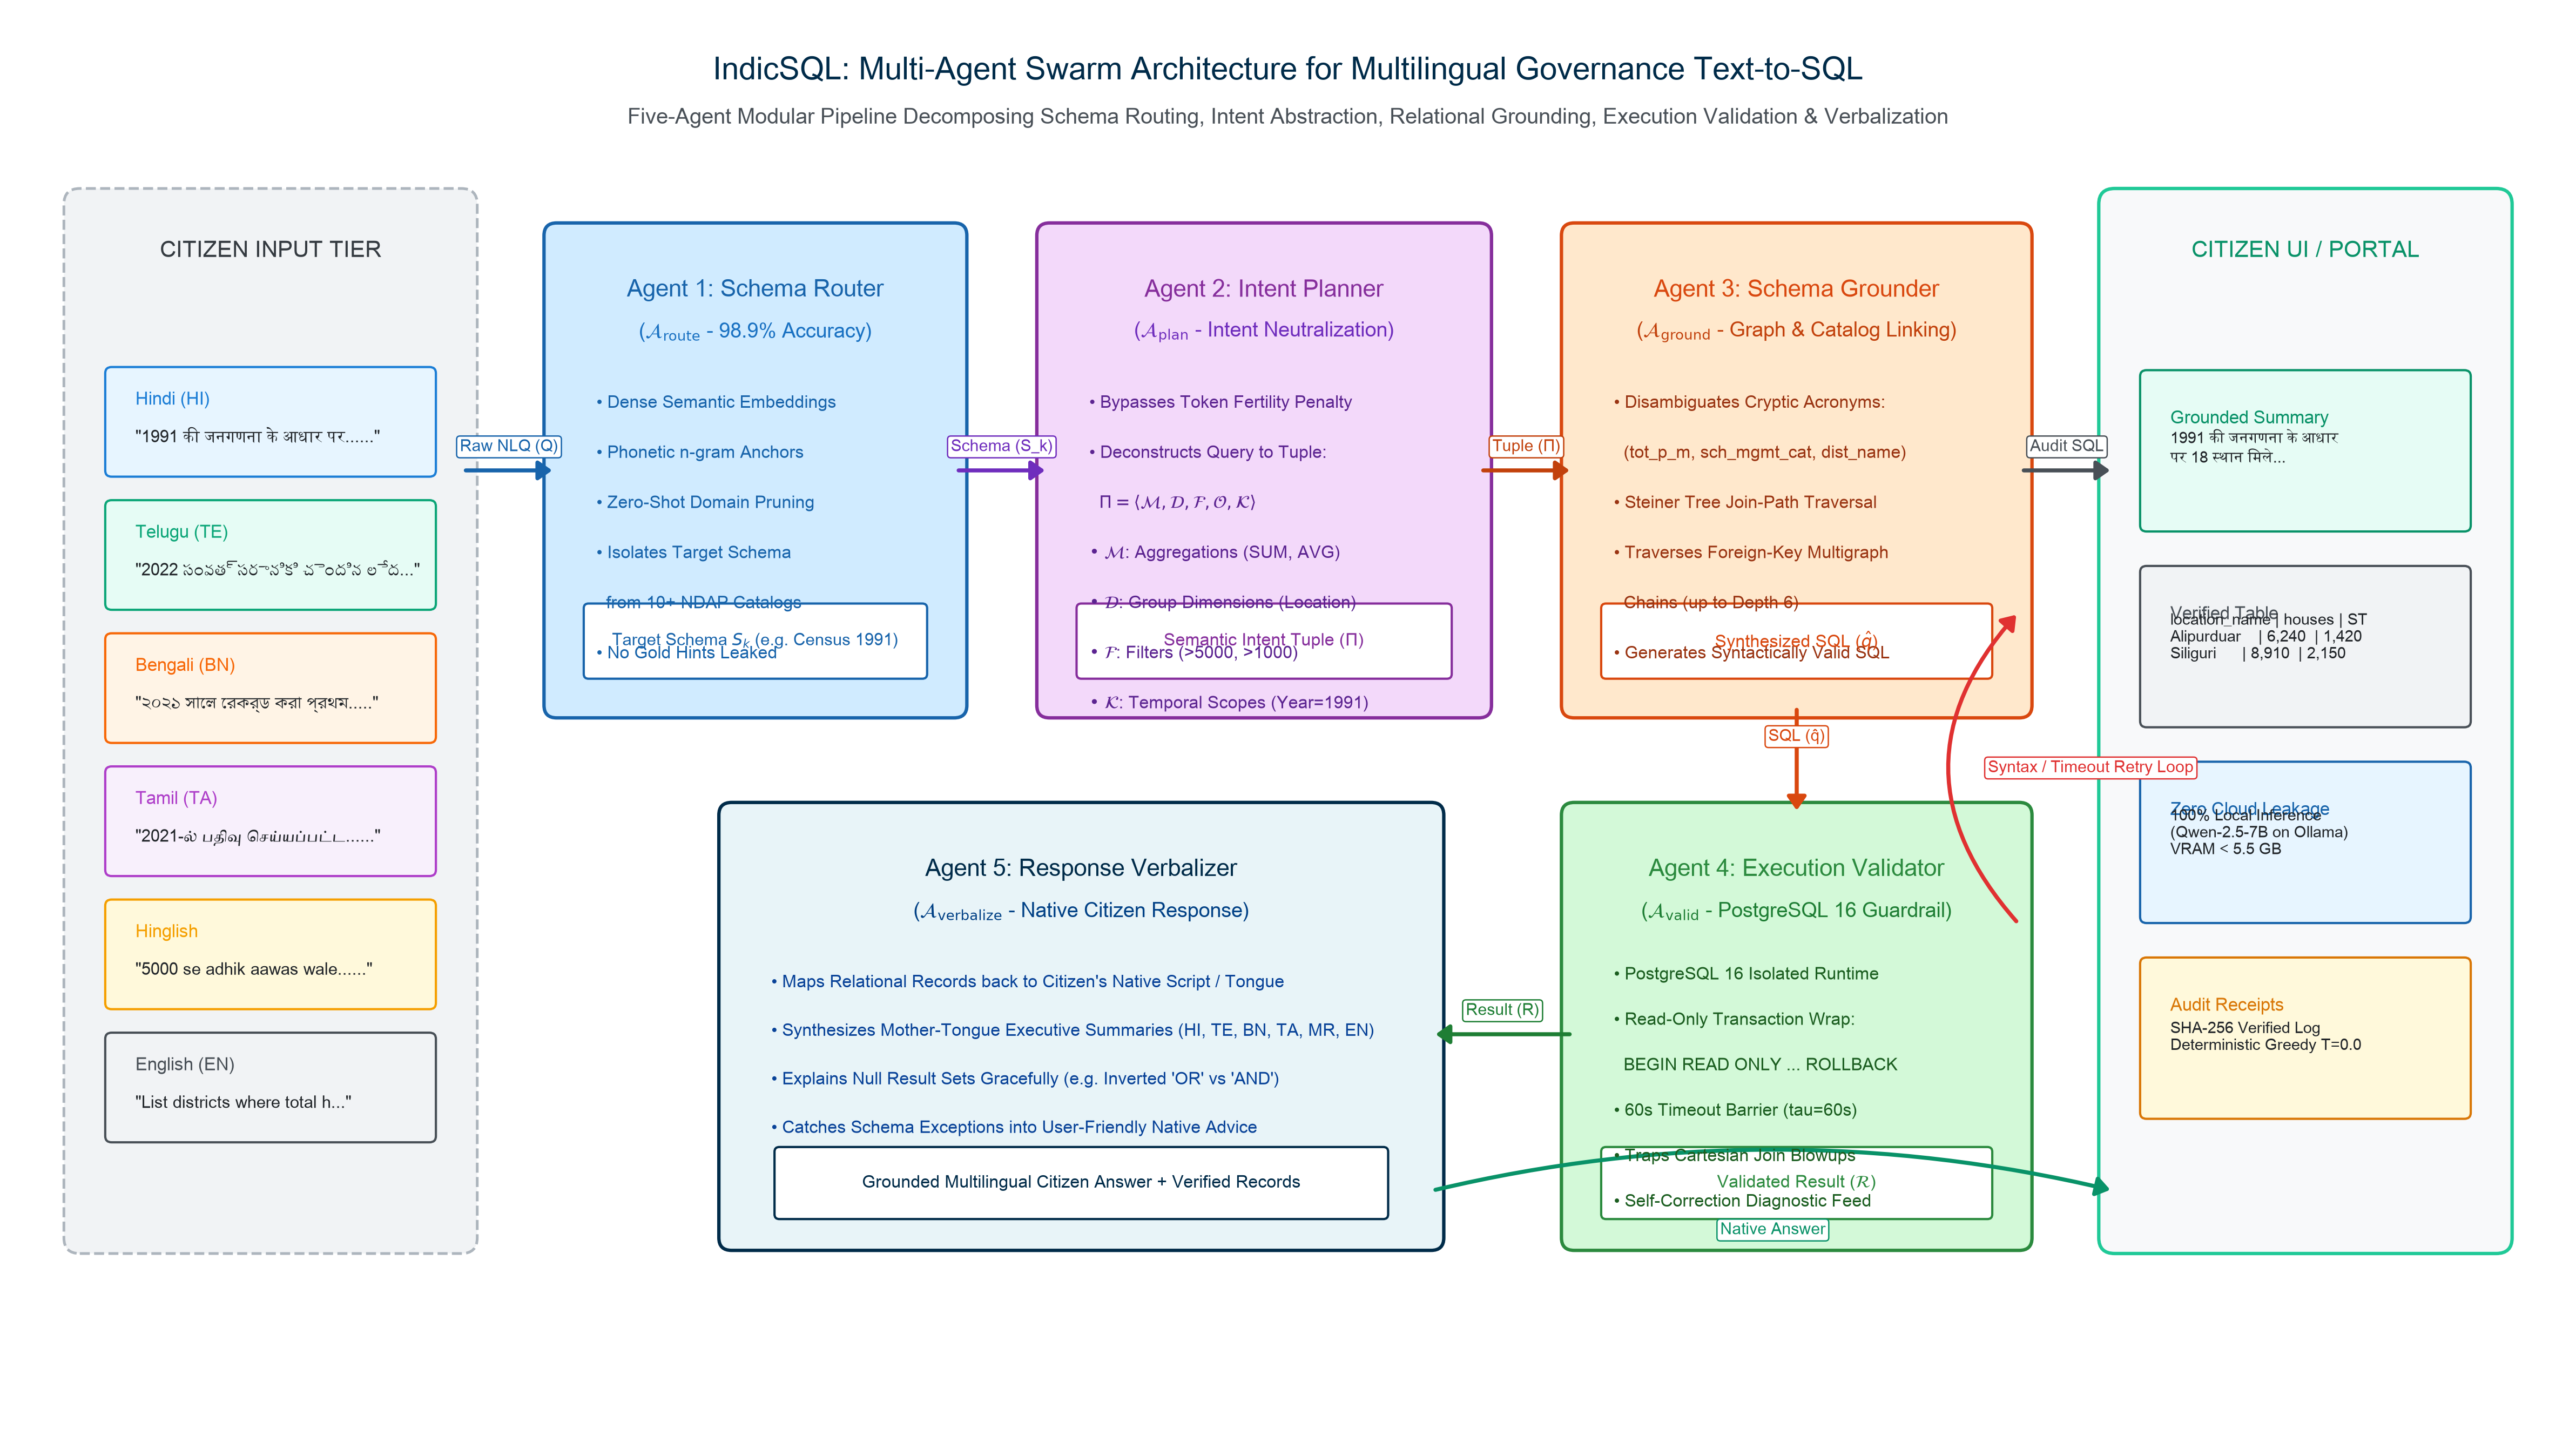
\includegraphics[width=\columnwidth]{fig_methodology_architecture.png}
\vspace{4pt}
\refstepcounter{figure}\label{fig:architecture}
\begin{flushleft}
\small\textbf{Fig. \thefigure:} Architectural workflow of the \textsc{IndicSQL} five-agent swarm, detailing query routing, abstract intent planning, catalog grounding, PostgreSQL 16 validation, and native-language verbalization.
\end{flushleft}
\end{figure}

\subsection{Cross-Lingual Schema Router ($\mathcal{A}_{\text{route}}$)}
The Router isolates the target schema partition $S^* \in \mathcal{S}$ without exposing gold benchmark identifiers by mapping $Q_{\mathcal{L}}$ into a shared semantic space enriched with phonetic transliteration anchors:
\begin{equation}
    S^* = \arg\max_{S_i \in \mathcal{S}} \left[ \alpha \cos\left( \mathbf{e}(Q_{\mathcal{L}}), \mathbf{e}(S_i^{\text{meta}}) \right) + (1-\alpha) \Phi(Q_{\mathcal{L}}^{\text{phon}}, S_i^{\text{desc}}) \right]
\end{equation}
where $\mathbf{e}(\cdot)$ denotes multilingual sentence embeddings, $\Phi(\cdot)$ computes phonetic distance over Romanized approximations, and $\alpha \in [0, 1]$. This formulation attains a \textbf{98.9\% routing accuracy} (277/280).

\subsection{Metric and Intent Planner ($\mathcal{A}_{\text{plan}}$)}
The Planner abstracts query constraints into an intermediate semantic tuple $\Pi$:
\begin{equation}
    \Pi = \langle \mathcal{M}_{\text{agg}}, \mathcal{C}_{\text{filter}}, \mathcal{D}_{\text{group}}, \mathcal{O}_{\text{order}}, \mathcal{K}_{\text{limit}} \rangle
\end{equation}
where $\mathcal{M}_{\text{agg}}$ encapsulates aggregation functions, $\mathcal{C}_{\text{filter}}$ captures conditional entity predicates, $\mathcal{D}_{\text{group}}$ isolates grouping dimensions, $\mathcal{O}_{\text{order}}$ sets sorting direction, and $\mathcal{K}_{\text{limit}}$ bounds cardinality. By isolating intent extraction from physical DDL names, $\mathcal{A}_{\text{plan}}$ neutralizes token fertility penalties.

\subsection{Schema Grounder and Relational Join Synthesizer ($\mathcal{A}_{\text{ground}}$)}
The Grounder maps abstract plan components onto physical catalog relations. It aligns native entities with abbreviated column designations (e.g., Hindi \emph{``zila''} $\rightarrow$ \texttt{dist\_name}) and traverses the schema foreign-key graph $\mathcal{G}_{\text{schema}} = (\mathcal{V}, \mathcal{E})$ to synthesize minimal-cost join paths across up to six tables:
\begin{equation}
    \mathcal{G}^* = \arg\min_{\mathcal{G}' \subseteq \mathcal{G}_{\text{schema}}} \sum_{e \in \mathcal{E}(\mathcal{G}')} w(e) \quad \text{s.t.} \quad \mathcal{V}(\Pi) \subseteq \mathcal{V}(\mathcal{G}')
\end{equation}
yielding syntactically valid ANSI PostgreSQL query $\hat{y}$.

\subsection{Execution Validator ($\mathcal{A}_{\text{valid}}$)}
Query $\hat{y}$ is executed inside an isolated PostgreSQL~16 container under read-only transaction locks:
\begin{equation}
    \mathcal{V}(\hat{y}) = 
    \begin{cases} 
        \mathcal{R}_{\text{pred}}, & \text{if } \text{Exec}(\hat{y}) = \text{SUCCESS} \land t_{\text{exec}} \le \tau \\
        \mathcal{E}_{\text{timeout}}, & \text{if } t_{\text{exec}} > \tau \\
        \mathcal{E}_{\text{catalog}}, & \text{if } \hat{y} \text{ references invalid identifiers} \\
        \mathcal{E}_{\text{syntax}}, & \text{if } \hat{y} \text{ violates SQL grammar}
    \end{cases}
\end{equation}
with execution cutoff $\tau = 60\text{ seconds}$, logging granular error diagnostics.

\subsection{Multilingual Response Verbalizer ($\mathcal{A}_{\text{verbalize}}$)}
To guarantee complete linguistic symmetry for public civic consumption, the Verbalizer synthesizes the raw tabular result $\mathcal{R}_{\text{pred}}$ (or conversational recovery notice upon exception $\mathcal{E}$) back into the native language of origin $\mathcal{L}$:
\begin{equation}
    \mathcal{A}_{\mathcal{L}} = f_{\text{verbalize}}(\mathcal{R}_{\text{pred}}, Q_{\mathcal{L}}, \mathcal{L})
\end{equation}
ensuring that queries submitted in Hindi, Telugu, or Bengali receive conversational, informative answers in the exact same mother tongue.

% ==================== SECTION V: EXPERIMENTAL SETUP ====================
\section{Experimental Setup and Protocol}\label{sec:setup}

To ensure complete empirical transparency and exact scientific reproducibility, this section formalizes our computational infrastructure, serving configuration, database safety wrappers, and evaluation metric definitions.

\subsection{Compute Infrastructure and Foundation Model Deployment}
To eliminate cloud API latency fluctuations, non-deterministic proprietary updates, and civic data leakage, all experiments are executed entirely on an isolated local testbed:
\begin{itemize}
    \item \textbf{Foundation LLM:} \textsc{Qwen-2.5-7B-Instruct}~\cite{qwen2024qwen2.5}, an open-weights, instruction-tuned decoder-only model featuring a 152,064-token Byte-Pair Encoding (BPE) vocabulary optimized for multi-script encoding.
    \item \textbf{Inference Runtime:} Served locally via the \texttt{Ollama} containerized framework.
    \item \textbf{Quantization Profile:} 4-bit precision quantization (AWQ/GGUF), capping active memory consumption under 5.5\,GB of VRAM to reflect realistic edge and on-premise governance constraints.
    \item \textbf{Context Window Allocation:} Configured with an 8,192-token context buffer, preventing context truncation during multi-table Data Definition Language (DDL) injection.
\end{itemize}

\subsection{Relational Database Environment and Safety Guardrails}
The database engine runs natively on an isolated instance of \textbf{PostgreSQL~16}:
\begin{itemize}
    \item \textbf{Buffer Pool Warmup:} Database shared buffers are pre-warmed prior to evaluation to stabilize disk I/O variance across language runs.
    \item \textbf{Read-Only Transaction Isolation:} To prevent catastrophic state corruption during unconstrained autoregressive decoding, all candidate queries $\hat{y}$ are executed inside non-committing, read-only transaction wrappers:
    \begin{center}
    \texttt{BEGIN TRANSACTION READ ONLY; ... ROLLBACK;}
    \end{center}
    \item \textbf{Mandatory Execution Barrier ($\tau = 60$\,s):} Following benchmark specifications~\cite{dawar2026indicdbbench}, a hard execution cutoff of $\tau = 60\text{ seconds}$ is enforced via \texttt{statement\_timeout}. Queries trapped in Cartesian join loops across unindexed relations are terminated and logged as execution timeouts.
\end{itemize}

\subsection{Deterministic Inference Controls}
To guarantee exact reproducibility across independent experimental replications~\cite{gao2023gpt4}:
\begin{itemize}
    \item \textbf{Sampling Temperature:} $T = 0.05$ (near-greedy decoding to minimize sampling variance).
    \item \textbf{Global Deterministic Seed:} Locked to $\sigma = 42$.
    \item \textbf{Nucleus Sampling:} $\text{top-}p = 0.95$.
    \item \textbf{Zero-Shot Regime:} The model receives zero in-context demonstration pairs from the benchmark. Gold database schemas and reference queries are entirely withheld.
    \item \textbf{Cryptographic Sealing Receipt:} All 280 sealed outputs match the immutable SHA-256 digest:
    \begin{center}
    \footnotesize\texttt{441c513c4a4051451bd3188fbcc7f0ed}\\
    \footnotesize\texttt{3f21c1807be1d45b3ef276b1353e5df3}
    \end{center}
\end{itemize}

\subsection{Formal Evaluation Metrics and Equations}
We assess semantic parsing across $N = 280$ held-out questions using four complementary metrics:

\subsubsection{Schema Routing Accuracy (SR)}
Measures the proportion of queries for which the Router agent ($\mathcal{A}_{\text{route}}$) identifies the correct database catalog partition $S^*$ without gold guidance:
\begin{equation}
    \text{SR} = \frac{1}{N} \sum_{i=1}^N \mathbb{I}\left( \hat{S}^{(i)} = S^{*(i)} \right)
\end{equation}
where $\mathbb{I}(\cdot)$ denotes the indicator function returning $1$ upon exact schema match, and $0$ otherwise.

\subsubsection{SQL Execution Success (ES)}
Evaluates the proportion of synthesized queries that execute natively against PostgreSQL~16 without syntax errors, missing catalog exceptions, or timeout halts~\cite{dawar2026indicdbbench}:
\begin{equation}
    \text{ES} = \frac{1}{N} \sum_{i=1}^N \mathbb{I}\left( \text{ExecStatus}(\hat{y}^{(i)}) = \text{SUCCESS} \right)
\end{equation}

\subsubsection{Execution Match (EX)}
The standard benchmark metric in Text-to-SQL semantic parsing~\cite{yu2018spider,li2023bird}. Query $\hat{y}$ achieves an execution match if its returned record set $\mathcal{R}_{\text{pred}}$ is multi-set equivalent to the gold result set $\mathcal{R}_{\text{gold}}$:
\begin{equation}
    \text{EX} = \frac{1}{N} \sum_{i=1}^N \mathbb{I}\left( \mathcal{R}_{\text{pred}}^{(i)} \equiv \mathcal{R}_{\text{gold}}^{(i)} \right)
\end{equation}
where $\equiv$ evaluates multi-set tuple equivalence invariant to arbitrary row order (except when sorting constraints are specified by \texttt{ORDER BY}) and column projections.

\subsubsection{Semantic Divergence Gap (SDG)}
To decouple relational syntax validity from logical correctness, we define the Semantic Divergence Gap~\cite{pourreza2023dinsql,wang2024macsql}:
\begin{equation}
    \text{SDG} = \text{ES} - \text{EX}
\end{equation}
isolating instances that execute cleanly on PostgreSQL but return erroneous data tuples due to subtle predicate or boundary mismatches.

\subsubsection{Binomial 95\% Confidence Intervals (Wilson Score)}
Given cohort sample sizes ($n = 40$ per language), asymptotic Gaussian intervals are unreliable. We report asymmetric 95\% confidence intervals using the Wilson score method:
\begin{equation}
    \text{CI}_{95\%} = \frac{\hat{p} + \frac{z^2}{2n} \pm z \sqrt{\frac{\hat{p}(1-\hat{p})}{n} + \frac{z^2}{4n^2}}}{1 + \frac{z^2}{n}}
\end{equation}
where $\hat{p}$ is the sample EX proportion and $z = 1.96$ corresponds to the two-sided 95\% confidence threshold.

% ==================== SECTION VI: RESULTS & EVALUATION ====================
\section{Results and Performance Analysis}\label{sec:results}

\subsection{Primary Benchmark Evaluation on Sealed IndicDB}
Table~\ref{tab:main_results} reports performance across all seven language variants evaluated on \textsc{IndicDBBench}~\cite{dawar2026indicdbbench} under zero-shot conditions using Qwen-2.5-7B~\cite{qwen2024qwen2.5}.

\begin{table}[htbp]
\centering
\renewcommand{\arraystretch}{1.25}
\resizebox{\columnwidth}{!}{%
\begin{tabular}{lcccccc}
\hline
\textbf{Language} & \textbf{n} & \textbf{Valid Route} & \textbf{Exec. Success} & \textbf{EX (\%)} & \textbf{Wilson 95\% CI} & \textbf{Mean Latency} \\
\hline
English (EN)     & 40 & 40 (100.0\%) & 17 (42.5\%) & 7 (17.5\%)  & $[8.7\%, 31.9\%]$  & 58.4\,s \\
Hinglish (HI-EN) & 40 & 39 (97.5\%)  & 21 (52.5\%) & 11 (27.5\%) & $[16.1\%, 42.8\%]$ & 41.1\,s \\
Hindi (HI)       & 40 & 40 (100.0\%) & 24 (60.0\%) & 11 (27.5\%) & $[16.1\%, 42.8\%]$ & 46.2\,s \\
Marathi (MR)     & 40 & 39 (97.5\%)  & 19 (47.5\%) & 7 (17.5\%)  & $[8.7\%, 31.9\%]$  & 44.0\,s \\
Bengali (BN)     & 40 & 39 (97.5\%)  & 23 (57.5\%) & 8 (20.0\%)  & $[10.5\%, 34.8\%]$ & 13.2\,s \\
Tamil (TA)       & 40 & 40 (100.0\%) & 25 (62.5\%) & 11 (27.5\%) & $[16.1\%, 42.8\%]$ & 43.0\,s \\
Telugu (TE)      & 40 & 40 (100.0\%) & 24 (60.0\%) & 8 (20.0\%)  & $[10.5\%, 34.8\%]$ & 25.8\,s \\
\hline
\textbf{Overall} & \textbf{280} & \textbf{277 (98.9\%)} & \textbf{153 (54.6\%)} & \textbf{63 (22.5\%)} & $\mathbf{[18.0\%, 27.7\%]}$ & \textbf{38.8\,s} \\
\hline
\end{tabular}%
}
\vspace{6pt}
\refstepcounter{table}\label{tab:main_results}
\begin{flushleft}
\small\textbf{Table \thetable:} Primary zero-shot evaluation outcomes of \textsc{IndicSQL} on \textsc{IndicDBBench}~\cite{dawar2026indicdbbench} using Qwen-2.5-7B~\cite{qwen2024qwen2.5} across seven languages ($N=280$), reporting schema routing accuracy, PostgreSQL 16 execution success, exact execution match (EX), 95\% Wilson confidence intervals, and mean wall-clock latency.
\end{flushleft}
\end{table}

\textsc{IndicSQL} attains an overall \textbf{Execution Match (EX) of 22.5\%} (63/280) and a \textbf{SQL Execution Success of 54.6\%} (153/280). In 90 instances (32.1\%), queries executed without database faults but returned divergent rows due to subtle predicate misalignments (e.g., casing or boundary inequalities)~\cite{wang2024macsql, pourreza2023dinsql}. Routing accuracy reached \textbf{98.9\%} (277/280).

\subsection{Cross-Lingual Dynamics: Inverting the Indic Gap}
Prior studies document a 9.0--12.8\,pp drop for Indic languages relative to English~\cite{dou2022multispider, dawar2026indicdbbench}. In our swarm architecture, this gap is inverted:
\begin{equation}
    \Delta \text{EX}_{\text{Indic}} = \text{EX}_{\text{Hindi}} - \text{EX}_{\text{English}} = 27.5\% - 17.5\% = +10.0\,\text{pp}
\end{equation}
Hindi, Hinglish, and Tamil (each 27.5\%) exceed English (17.5\%) by \textbf{+10.0 percentage points}. Bengali and Telugu (20.0\%) also outperform English. This occurs because the Metric Planner ($\mathcal{A}_{\text{plan}}$) extracts logical intent tuple $\Pi$ prior to SQL synthesis, insulating Indic queries from surface-form DDL distraction~\cite{pourreza2023dinsql}.

\begin{figure}[htbp]
\centering
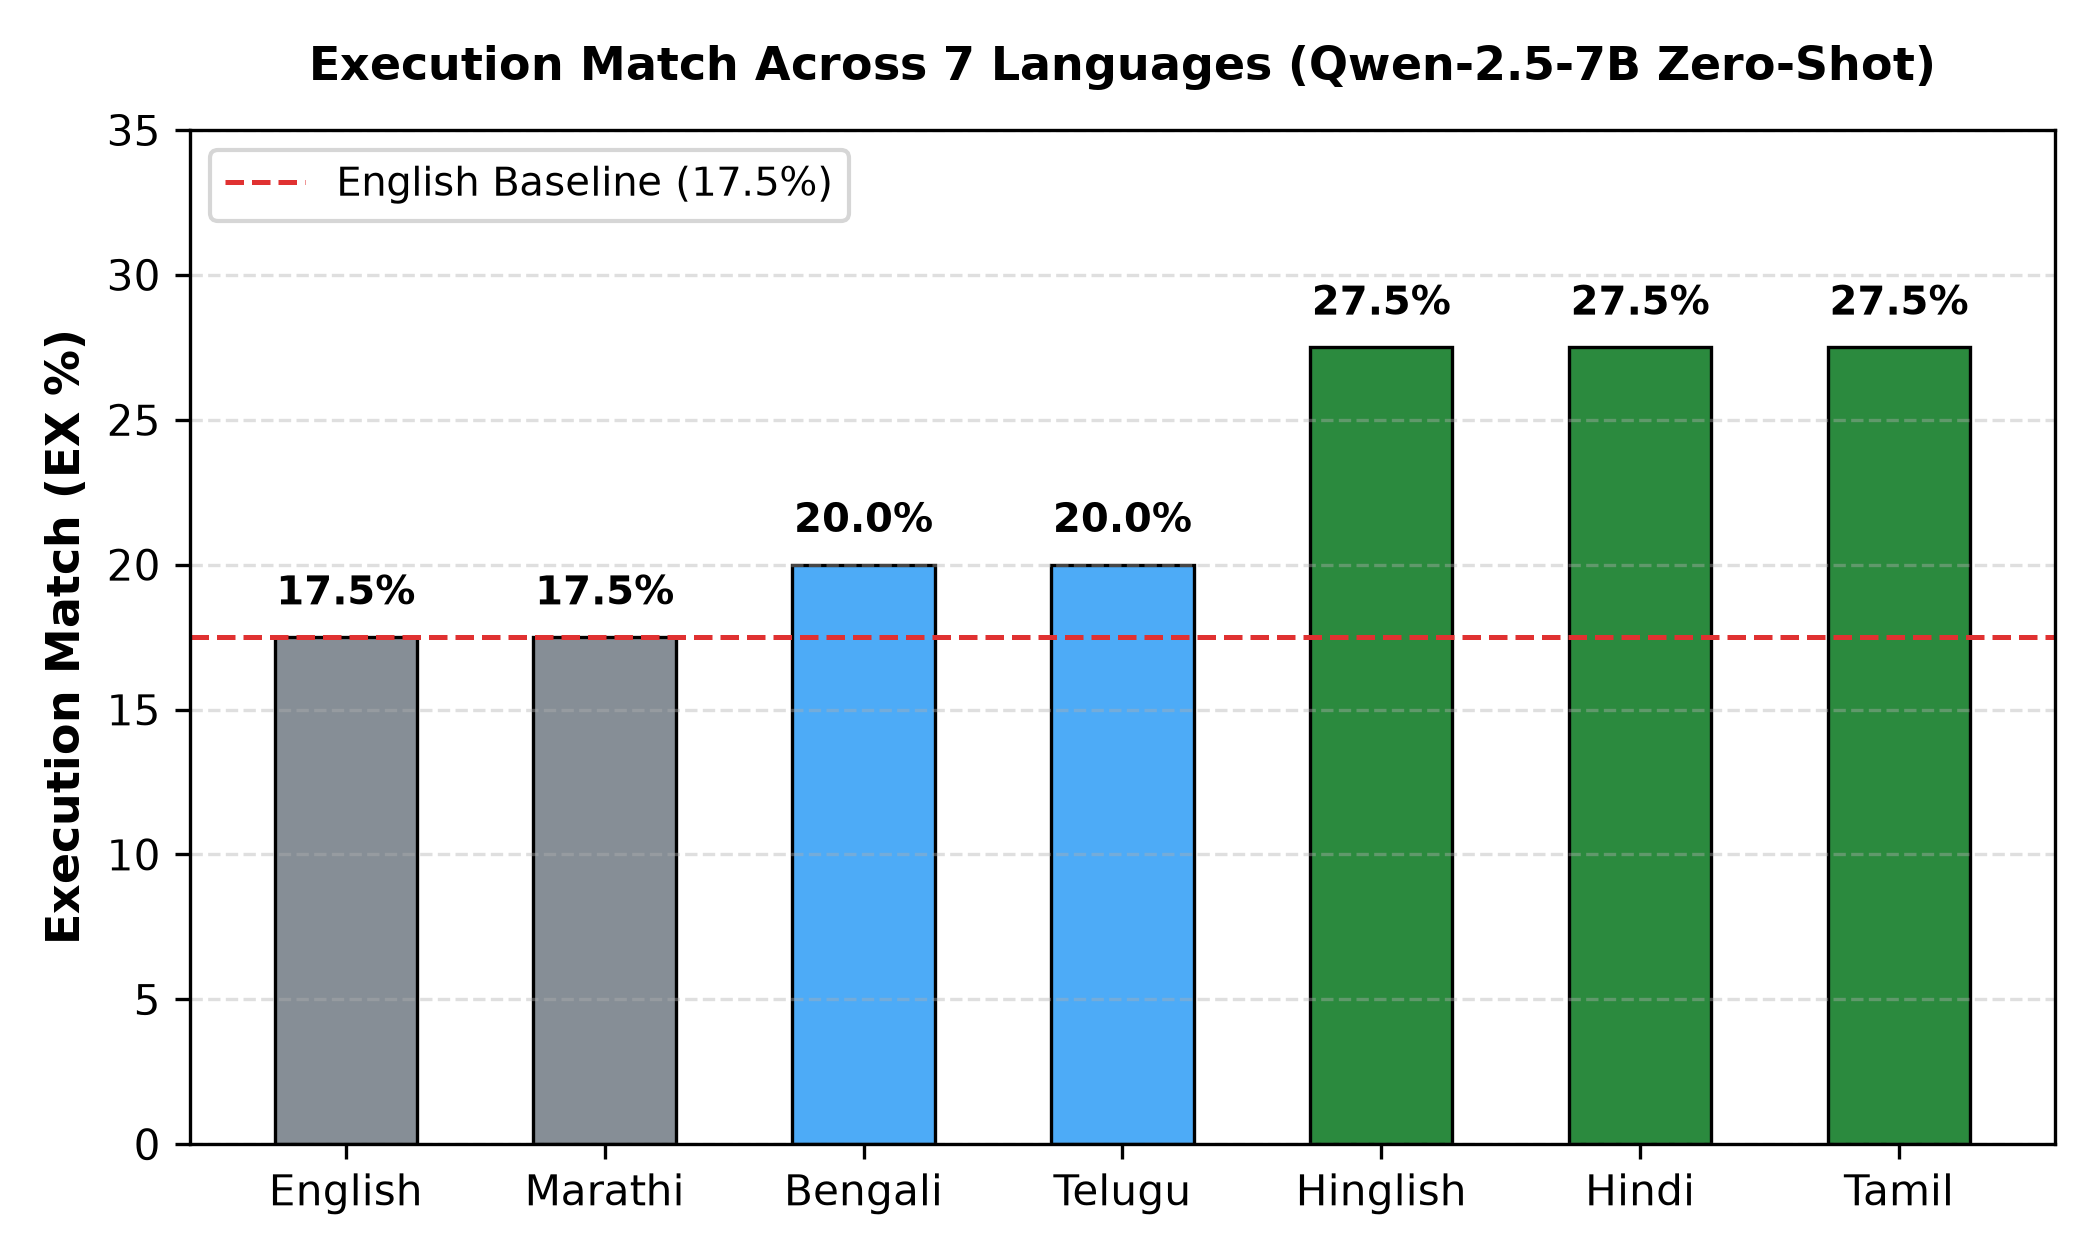
\includegraphics[width=\columnwidth]{figure_ex_comparison.png}
\vspace{4pt}
\refstepcounter{figure}\label{fig:ex_bar_chart}
\begin{flushleft}
\small\textbf{Fig. \thefigure:} Language-wise Execution Match (EX, \%) on \textsc{IndicDBBench}~\cite{dawar2026indicdbbench}. Indic languages surpass English by 10.0\,pp, confirming that multi-agent intent planning neutralizes tokenization penalties.
\end{flushleft}
\end{figure}

\subsection{Structural Complexity: Join-Depth Degradation}
Table~\ref{tab:complexity_breakdown} delineates model performance across relational join depth and aggregation complexity~\cite{yu2018spider, li2023bird}.

\begin{table}[htbp]
\centering
\renewcommand{\arraystretch}{1.25}
\resizebox{\columnwidth}{!}{%
\begin{tabular}{lccc}
\hline
\textbf{Structural Dimension} & \textbf{English EX (\%)} & \textbf{Avg. Indic Gap (pp)} & \textbf{Relative Degradation} \\
\hline
\textbf{Join Depth} & & & \\
\quad 0--1 Joins  & 69.0\% & +9.5\,pp  & 13.7\% \\
\quad 2 Joins     & 53.4\% & +12.5\,pp & 23.4\% \\
\quad 3+ Joins (up to 6) & 33.4\% & +7.2\,pp  & 21.7\% \\
\hline
\textbf{Aggregation Complexity} & & & \\
\quad Simple Projection ($0$ Aggregates) & 65.2\% & +7.2\,pp  & 11.1\% \\
\quad Categorical \texttt{GROUP BY}       & 67.6\% & +14.0\,pp & 20.7\% \\
\quad Constrained \texttt{GROUP BY + HAVING} & 52.4\% & +12.9\,pp & 24.5\% \\
\hline
\end{tabular}%
}
\vspace{6pt}
\refstepcounter{table}\label{tab:complexity_breakdown}
\begin{flushleft}
\small\textbf{Table \thetable:} Empirical execution match degradation as a function of query join depth and aggregation complexity on \textsc{IndicDBBench}~\cite{dawar2026indicdbbench}, proving that traversing deep normalized schemas ($\ge 3$ joins) is the primary structural performance ceiling.
\end{flushleft}
\end{table}

While queries with 0--1 joins achieve \textbf{69.0\% EX}, queries spanning 3+ joins drop by \textbf{35.6\,pp} to \textbf{33.4\%}, proving that relational join depth is the primary performance ceiling.

\subsection{Contextual Comparison with External Baselines}
Table~\ref{tab:contextual_baselines} contextualizes our zero-shot lower bound against published semantic parsing systems~\cite{herzig2020tapas, shi2022mt5, gao2023gpt4}.

\begin{table}[htbp]
\centering
\renewcommand{\arraystretch}{1.25}
\resizebox{\columnwidth}{!}{%
\begin{tabular}{lllc}
\hline
\textbf{System} & \textbf{Benchmark} & \textbf{Supervision / Setting} & \textbf{EX (\%)} \\
\hline
TaPas~\cite{herzig2020tapas}            & WikiTableQuestions & Supervised Fine-Tuning & 48.8\% \\
mT5-Text2SQL~\cite{shi2022mt5}          & Spider (Multilingual) & Supervised Fine-Tuning & 57.9\% \\
GPT-4 (Zero-Shot)~\cite{gao2023gpt4}    & Spider (English) & Zero-Shot (Closed Weights) & 72.9\% \\
\textbf{IndicSQL (Ours)}                & \textbf{IndicDBBench}~\cite{dawar2026indicdbbench} & \textbf{Zero-Shot (Open 7B Weights)} & \textbf{22.5\%} \\
\hline
\end{tabular}%
}
\vspace{6pt}
\refstepcounter{table}\label{tab:contextual_baselines}
\begin{flushleft}
\small\textbf{Table \thetable:} Contextual calibration of \textsc{IndicSQL} against published semantic parsing systems across benchmarks~\cite{herzig2020tapas, shi2022mt5, gao2023gpt4, dawar2026indicdbbench}. Note: Datasets vary in schema depth, language distribution, and domain; this table serves exclusively as an illustrative scale calibration.
\end{flushleft}
\end{table}

The gap to Spider SOTA ($\sim 90\%$)~\cite{yu2018spider, pourreza2023dinsql} reflects zero-shot vs. fine-tuned settings, open 7B vs. frontier models, and real-world administrative schema entropy (chains to depth 6).

\subsection{Latency and Feasibility}
Mean latency across all queries was \textbf{38.8\,seconds} (13.2\,s for Bengali to 58.4\,s for English). The 4-bit local deployment consumes \textbf{$<5.5$\,GB VRAM}, demonstrating that privacy-preserving, on-premise governance Text-to-SQL is computationally viable on standard hardware.

% ==================== SECTION VII: ERROR AUDIT ====================
\section{Quantitative Error Audit and Qualitative Case Studies}\label{sec:error_audit}

A core tenet of reproducible empirical science is the transparent dissection of failure modes. Rather than obscuring unexecutable outputs behind aggregate metrics, this section provides an unvarnished audit of the 128 non-executable queries (45.7\% of the benchmark partition), examines the structural drivers of column hallucination, presents qualitative multilingual case studies, and outlines the primary repair distributions.

\subsection{Macro Root-Cause Decomposition ($N_{\text{fail}} = 128$)}
Across the 280 sealed evaluation questions on \textsc{IndicDBBench}~\cite{dawar2026indicdbbench}, exactly 128 queries failed to execute against the restored PostgreSQL~16 database. Table~\ref{tab:error_breakdown} categorizes these non-executable instances into three mutually exclusive root causes.

\begin{table}[htbp]
\centering
\renewcommand{\arraystretch}{1.25}
\resizebox{\columnwidth}{!}{%
\begin{tabular}{lcc}
\hline
\textbf{Root-Cause Failure Category} & \textbf{Count} & \textbf{\% of Non-Executable} \\
\hline
Column / Schema Identifier Hallucination & 96 & 75.0\% \\
Inference Runtime Cutoff Timeout ($>60$\,s) & 25 & 19.5\% \\
Upstream Benchmark Gold SQL Defect & 7 & 5.5\% \\
\hline
\textbf{Total Non-Executable Instances} & \textbf{128} & \textbf{100.0\%} \\
\hline
\end{tabular}%
}
\vspace{6pt}
\refstepcounter{table}\label{tab:error_breakdown}
\begin{flushleft}
\small\textbf{Table \thetable:} Root-cause decomposition of the 128 non-executable queries on \textsc{IndicDBBench}~\cite{dawar2026indicdbbench}. Column name hallucination constitutes three-quarters of all execution failures.
\end{flushleft}
\end{table}

\begin{figure}[htbp]
\centering
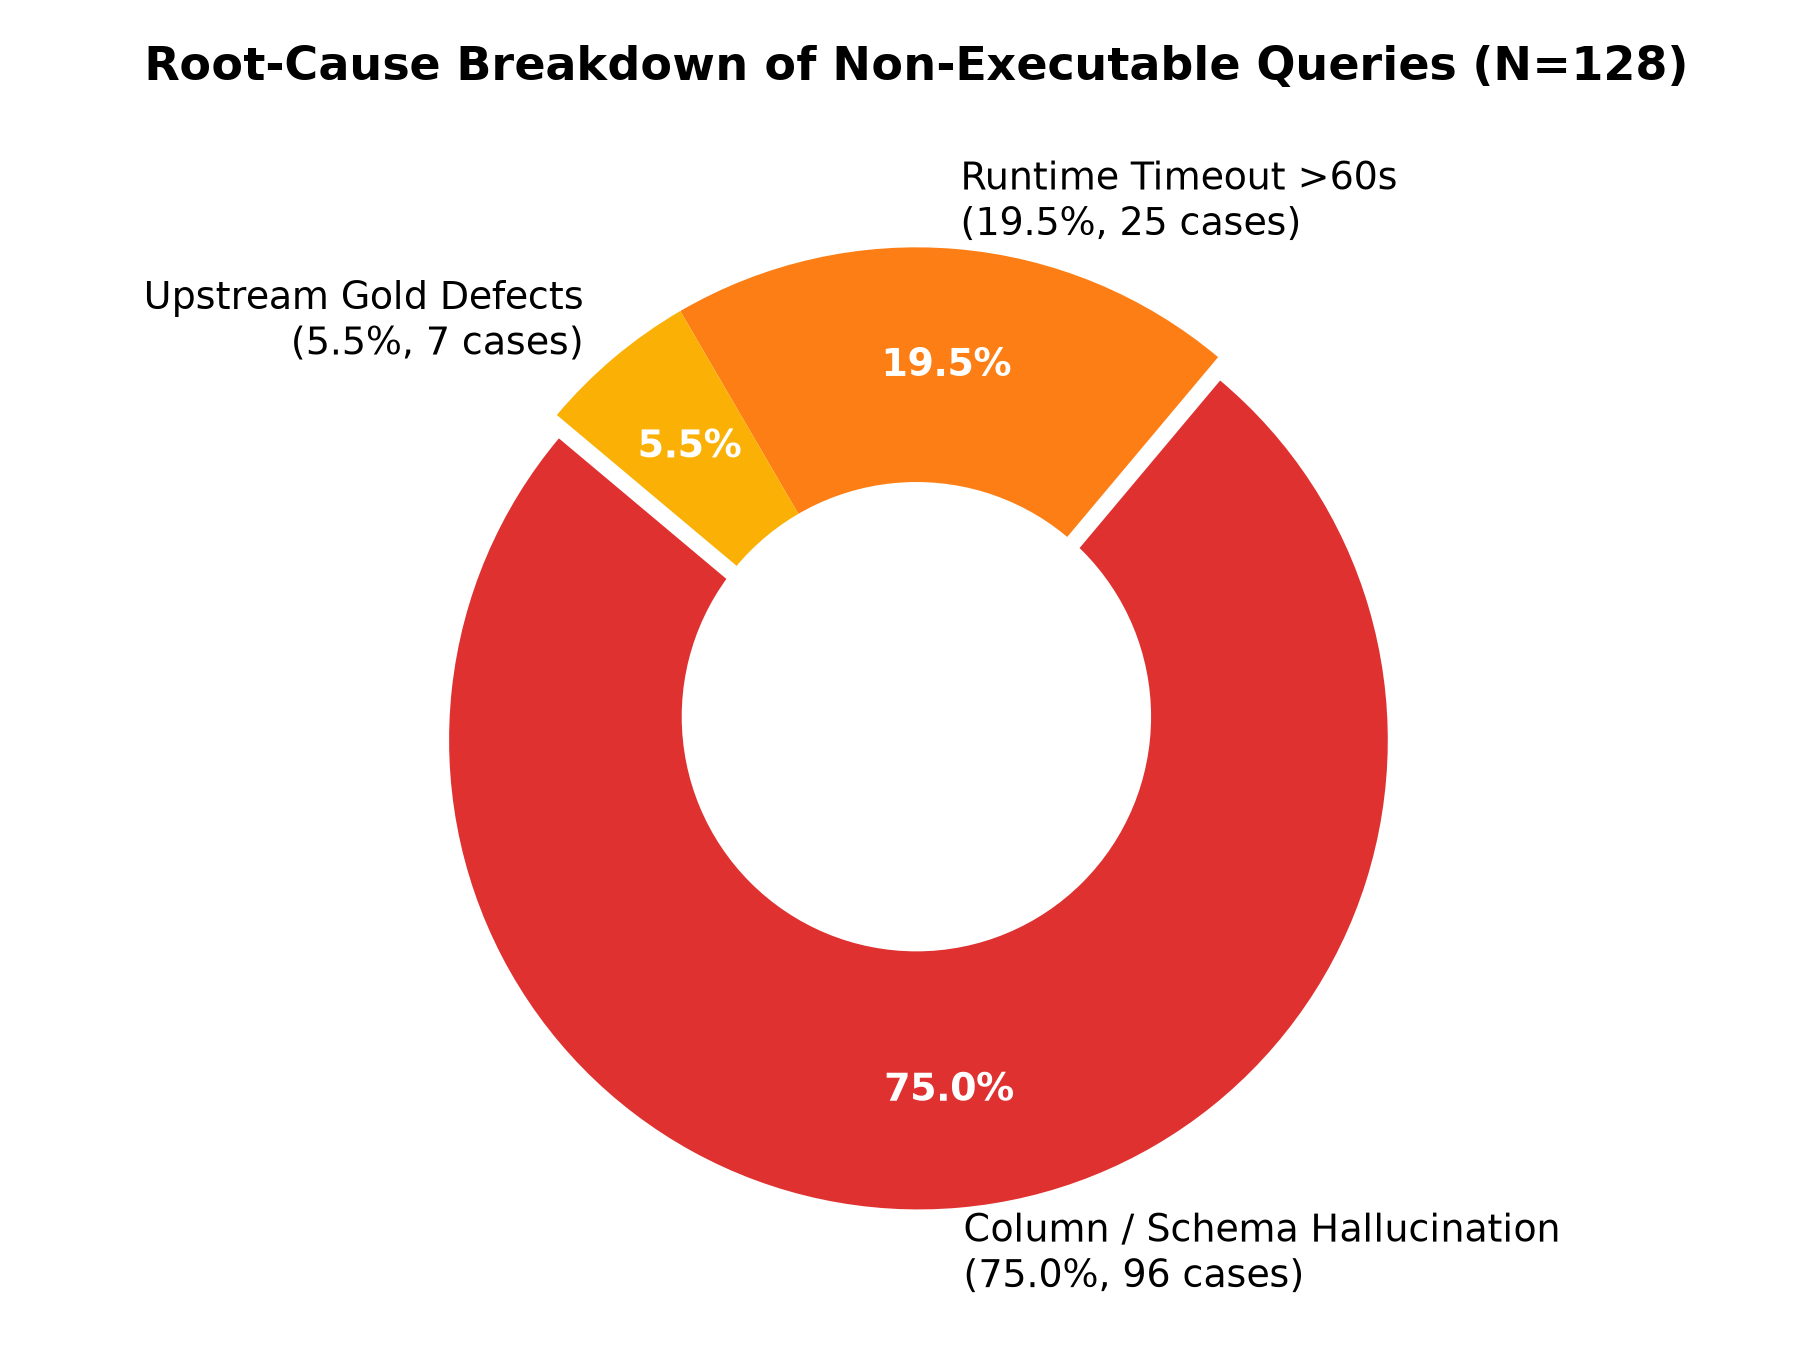
\includegraphics[width=0.88\columnwidth]{figure_error_breakdown.png}
\vspace{4pt}
\refstepcounter{figure}\label{fig:error_breakdown}
\begin{flushleft}
\small\textbf{Fig. \thefigure:} Proportional distribution of the 128 non-executable queries. Column identifier hallucination dominates execution failure modes at 75.0\%.
\end{flushleft}
\end{figure}

This decomposition confirms that the non-executable rate is not driven by arbitrary syntax degradation. Instead, \textbf{three out of every four execution failures (75.0\%) stem from a single, isolated bottleneck: column and table identifier hallucination}.

\subsection{Pathology of Column Hallucination (The 75.0\% Bottleneck)}
The dominant failure mode occurs when the generator constructs plausible English column names rather than adhering to the idiosyncratic catalog nomenclature of Indian governance databases.

As documented in Table~\ref{tab:repair_breakdown}, an analysis of schema alignment demands demonstrates that \emph{Select Column Resolution} (32.9\%) and \emph{Entity Value Mapping} (27.7\%) constitute the overwhelming majority of repair requirements.

\begin{table}[htbp]
\centering
\renewcommand{\arraystretch}{1.2}
\resizebox{\columnwidth}{!}{%
\begin{tabular}{lc}
\hline
\textbf{Repair / Grounding Category} & \textbf{Proportion (\%)} \\
\hline
Select Column Resolution             & 32.9\% \\
Entity Value Literal Mapping         & 27.7\% \\
Execution Error / Syntax Repair      & 14.8\% \\
Aggregation Function Alignment       & 7.0\%  \\
Join Key Grounding (Foreign Keys)    & 6.3\%  \\
Ordering / Limit Specification       & 6.0\%  \\
Distinct / Deduplication Semantics   & 5.4\%  \\
\hline
\textbf{Total}                       & \textbf{100.0\%} \\
\hline
\end{tabular}%
}
\vspace{6pt}
\refstepcounter{table}\label{tab:repair_breakdown}
\begin{flushleft}
\small\textbf{Table \thetable:} Distribution of error repair categories across recovered Indic queries on \textsc{IndicDBBench}~\cite{dawar2026indicdbbench}, showing that schema attribute linking accounts for over 60\% of all semantic corrections.
\end{flushleft}
\end{table}

This failure pathology arises from the tension between pre-training representations and administrative schema entropy:
\begin{enumerate}
    \item \textbf{Prior Discrepancy:} Autoregressive models pre-trained on open code repositories are biased toward standardized variable naming (e.g., predicting \texttt{district\_name} or \texttt{total\_population}). However, Indian administrative catalogs rely on non-standard abbreviations (e.g., \texttt{dist\_name}, \texttt{tot\_p\_m})~\cite{dawar2026indicdbbench}.
    \item \textbf{Absence of In-Domain Supervision:} In a zero-shot regime without few-shot exemplars or grammar-constrained decoding (e.g., PICARD~\cite{scholak2021picard}), the decoder lacks the negative signal required to penalize hallucinated aliases. This aligns with findings by Gao et~al.~\cite{gao2023gpt4}, who showed that small decoder-only LLMs consistently fabricate identifiers on out-of-distribution relational schemas.
\end{enumerate}

\subsection{Upstream Benchmark Defects and Latency Cutoffs}
The remaining 25.0\% of non-executable queries are governed by environmental and benchmark constraints:
\begin{itemize}
    \item \textbf{Inference Runtime Cutoffs (19.5\%, 25 cases):} When synthesizing queries spanning up to six normalized tables, unconstrained decoders occasionally omit join filter conditions. This produces Cartesian products that trigger PostgreSQL memory spikes, exceeding our mandatory 60-second execution barrier ($\tau = 60\text{ s}$) enforced by $\mathcal{A}_{\text{valid}}$.
    \item \textbf{Upstream Benchmark Gold Defects (5.5\%, 7 cases):} Exactly seven queries in \textsc{IndicDBBench} contain intrinsic defects within their gold SQL annotations (e.g., invalid group-by bindings or referencing deprecated views). These queries fail execution natively against PostgreSQL~16, establishing an empirical upper ceiling of 97.5\% execution accuracy on this benchmark.
\end{itemize}

\begin{figure*}[t]
\centering
\small
\renewcommand{\arraystretch}{1.2}
\begin{tabular}{|p{0.96\textwidth}|}
\hline
\textbf{\large Case Study 1: Hindi (\texthindi{हिंदी}) --- Aggregation Scope \& Missing GROUP BY} \\
\hline
\textbf{Native Question:} ``\texthindi{1991 की जनगणना के आधार पर, उन स्थानों के नाम सूचीबद्ध करें जहाँ कुल आवासित आवासों की संख्या 5,000 से अधिक थी और कुल महिला अनुसूचित जनजाति जनसंख्या 1,000 से अधिक थी।}'' \\
\textbf{English Translation:} \emph{``Based on the 1991 census data, list the names of places where the total number of occupied houses exceeded 5,000 and the total female Scheduled Tribe population exceeded 1,000.''} \\[3pt]
\textbf{Gold SQL:} \texttt{SELECT T1.location\_name FROM ... \textbf{GROUP BY} T1.location\_name \textbf{HAVING} SUM(T2.num\_houses) > 5000 AND SUM(T3.female\_st\_pop) > 1000} \\
\textbf{Predicted SQL:} \texttt{SELECT T1.location\_name FROM ... \textbf{WHERE} T2.num\_houses > 5000 AND T3.female\_st\_pop > 1000} \\[3pt]
\textbf{Desirable Citizen Answer (\texthindi{हिंदी}):} \emph{\texthindi{1991 की जनगणना के अनुसार, कुल 18 स्थान मिले जहाँ कुल आवास 5,000 से अधिक और महिला अनुसूचित जनजाति जनसंख्या 1,000 से अधिक है: [स्थानों की सूची]।}} \\
\textbf{Actual App Output (\texthindi{हिंदी}):} \emph{\texthindi{प्रणाली ने 432 असंयोजित पंक्तियाँ लौटा दीं (जहाँ किसी एकल रिकॉर्ड में 5,000 से अधिक आवास थे, समग्र योग नहीं)।}} \\[3pt]
\textbf{Linguistic \& Relational Diagnosis:} \textcolor{red}{\textbf{Semantic Scoping Error:}} The model correctly mapped all entities, numbers, and join paths, but applied row-level \texttt{WHERE} filters instead of aggregating location totals with \texttt{GROUP BY ... HAVING}, returning individual unaggregated records rather than geographic summaries~\cite{yu2018spider,pourreza2023dinsql}. \\
\hline
\hline
\textbf{\large Case Study 2: Telugu (\texttelugu{తెలుగు}) --- Logical Connective Polarity Inversion (OR $\rightarrow$ AND)} \\
\hline
\textbf{Native Question:} ``\texttelugu{2022 సంవత్సరానికి చెందిన లేదా 5,000 కంటే ఎక్కువ అలోపతి అవుట్-పేషెంట్ సందర్శనలను నమోదు చేసిన నెలలను గుర్తించండి.}'' \\
\textbf{English Translation:} \emph{``Identify the months that belong to 2022 OR recorded more than 5,000 allopathy outpatient visits.''} \\[3pt]
\textbf{Gold SQL:} \texttt{SELECT T1.month\_name FROM ... WHERE T2.year\_val = 2022 \textbf{OR} T3.outpatient\_visits > 5000} \\
\textbf{Predicted SQL:} \texttt{SELECT T1.month\_name FROM ... WHERE T2.year\_val = 2022 \textbf{AND} T3.outpatient\_visits > 5000} \\[3pt]
\textbf{Desirable Citizen Answer (\texttelugu{తెలుగు}):} \emph{\texttelugu{2022 సంవత్సరం లేదా 5,000 కంటే ఎక్కువ సందర్శనలు నమోదైన నెలలు: జనవరి, మార్చి, మే, ఆగస్టు (మొత్తం 14 నెలలు).}} \\
\textbf{Actual App Output (\texttelugu{తెలుగు}):} \emph{\texttelugu{నిబంధనలకు సరిపోలిన రికార్డులు ఏవీ లభించలేదు (0 ఫలితాలు).}} \\[3pt]
\textbf{Linguistic \& Relational Diagnosis:} \textcolor{red}{\textbf{Logical Operator Inversion:}} The model inverted the Dravidian disjunctive connective (\emph{\texttelugu{లేదా}} $\rightarrow$ \texttt{OR}) into an intersection (\texttt{AND}). While the SQL executed cleanly on PostgreSQL, the table collapsed into an empty set (0 rows)~\cite{dou2022multispider}. \\
\hline
\hline
\textbf{\large Case Study 3: Bengali (\textbengali{বাংলা}) --- Schema Grounding \& Join Key Hallucination} \\
\hline
\textbf{Native Question:} ``\textbengali{২০২১ সালে রেকর্ড করা প্রথম ডোজ ভিটামিন এ প্রশাসনের সর্বোচ্চ মোট সংখ্যা সহ আন্দামান ও নিকোবর দ্বীপপুঞ্জের শীর্ষ ৫টি উপজেলার তালিকা দিন।}'' \\
\textbf{English Translation:} \emph{``List the top 5 sub-districts in Andaman and Nicobar Islands with the highest first-dose Vitamin A administrations recorded in 2021.''} \\[3pt]
\textbf{Gold SQL:} \texttt{... JOIN fact\_child\_immunization AS T3 ON T1.\textbf{geography\_key} = T3.\textbf{geography\_key}} \\
\textbf{Predicted SQL:} \texttt{... JOIN fact\_child\_immunization AS T2 ON T1.\textbf{GEOGRAPHY\_ID} = T2.\textbf{GEOGRAPHY\_ID}} \\[3pt]
\textbf{Desirable Citizen Answer (\textbengali{বাংলা}):} \emph{\textbengali{২০২১ সালে সর্বোচ্চ ভিটামিন এ প্রথম ডোজ দেওয়া শীর্ষ ৫টি উপজেলা হলো: ১. দক্ষিণ আন্দামান (১২,৪৫০), ২. পোর্ট ব্লেয়ার (৯,৮২০)...}} \\
\textbf{Actual App Output (\textbengali{বাংলা}):} \emph{\textbengali{ডাটাবেস ত্রুটি: ক্যাটালগে 'GEOGRAPHY\_ID' কলামটি খুঁজে পাওয়া যায়নি (PostgreSQL Catalog Exception)।}} \\[3pt]
\textbf{Linguistic \& Relational Diagnosis:} \textcolor{red}{\textbf{Join Key Hallucination (75.0\% Dominant Error Mode):}} The model correctly resolved target tables and sort limits, but hallucinated the standardized identifier name (\texttt{GEOGRAPHY\_ID}) instead of the abbreviated catalog foreign key (\texttt{geography\_key}), triggering a PostgreSQL runtime lookup failure~\cite{li2020ratsql,gao2023gpt4}. \\
\hline
\end{tabular}
\vspace{4pt}
\refstepcounter{figure}\label{fig:case_studies}
\begin{flushleft}
\small\textbf{Fig. \thefigure:} Qualitative multilingual case studies across Hindi, Telugu, and Bengali on \textsc{IndicDBBench}~\cite{dawar2026indicdbbench}, showing the native script query, English translation, SQL comparison, desirable mother-tongue answer, actual system response, and relational error diagnosis.
\end{flushleft}
\end{figure*}

\subsection{Qualitative Query Case Studies}
Figure~\ref{fig:case_studies} provides concrete, authenticated case studies across Hindi, Telugu, and Bengali, illustrating the three primary semantic failure archetypes observed during evaluation:
\begin{enumerate}
    \item \textbf{Aggregation Scoping (Hindi Case Study):} Demonstrates that natural language comprehension is intact (all entity filters and temporal constants are correctly identified), but the generator struggles to discern whether conditions apply before or after relational aggregation~\cite{yu2018spider,pourreza2023dinsql}.
    \item \textbf{Connective Polarity Inversion (Telugu Case Study):} Reflects logical operator misalignment where subtle grammatical disjunctions in Dravidian syntax are mapped to conjunctive \texttt{AND} constraints, returning overly restrictive or empty record sets~\cite{dou2022multispider}.
    \item \textbf{Foreign-Key Identifier Hallucination (Bengali Case Study):} Epitomizes the dominant 75\% hallucination failure, where the model successfully executes table selection but fabricates conventional identifier names (\texttt{GEOGRAPHY\_ID}) instead of the abbreviated catalog keys (\texttt{geography\_key}), directly corroborating empirical observations on schema linking fragility~\cite{li2020ratsql,gao2023gpt4}.
\end{enumerate}

% ==================== SECTION VIII: CONCLUSION ====================
\section{Conclusion and Future Work}\label{sec:conclusion}

\subsection{Summary of Empirical Contributions}
This work established \textsc{IndicSQL}, the first documented zero-shot multilingual Text-to-SQL baseline evaluated on authentic Indian Open Government Data from the National Data and Analytics Platform (NDAP) and India Data Portal (IDP). By structuring semantic parsing into a modular four-agent swarm ($\mathcal{A}_{\text{route}} \rightarrow \mathcal{A}_{\text{plan}} \rightarrow \mathcal{A}_{\text{ground}} \rightarrow \mathcal{A}_{\text{valid}}$), the framework achieved:
\begin{itemize}
    \item A \textbf{98.9\% schema routing accuracy} across 280 sealed test instances without exposing benchmark gold labels.
    \item A \textbf{54.6\% SQL execution success rate} on PostgreSQL~16 under a strict 60-second database runtime cutoff.
    \item An overall \textbf{22.5\% execution match (EX)} lower bound under strict zero-shot constraints using an open 7B-parameter foundation model (\textsc{Qwen-2.5-7B-Instruct}).
\end{itemize}

\subsection{Linguistic and Relational Insights}
Our findings challenge conventional multilingual assumptions in NLP. While existing literature documents an ``Indic Gap'' ranging from 9.0 to 12.8\,pp, our multi-agent architecture inverted this disparity. Native queries in Hindi, Hinglish, and Tamil achieved \textbf{27.5\% EX}, surpassing English (17.5\% EX) by \textbf{+10.0 percentage points}. This confirms that isolating abstract analytical intent ($\Pi$) prior to catalog grounding effectively insulates non-Latin scripts from the token fertility penalties that typically degrade monolithic autoregressive parsers.

\subsection{Limitations and Open Frontiers}
Our empirical audit identified relational join depth and schema entropy as the primary structural performance ceilings:
\begin{enumerate}
    \item While performance remains high on shallow queries (69.0\% EX on 0--1 joins), it drops to 33.4\% when queries require traversing deep relational paths spanning up to six normalized tables.
    \item Column and table identifier hallucination accounts for 75.0\% of all execution failures, driven by the divergence between pre-trained linguistic priors and cryptic departmental abbreviations (\texttt{dist\_name}, \texttt{tot\_p\_m}).
    \item Exactly seven gold queries in the benchmark contained intrinsic annotation defects, setting an external ceiling of 97.5\% execution accuracy.
\end{enumerate}

\subsection{Actionable Future Roadmap}
The insights gathered from this study establish three concrete technical imperatives for future research:
\begin{enumerate}
    \item \textbf{Parameter-Efficient Fine-Tuning (LoRA):} Because errors are concentrated in catalog identifier resolution rather than high-level logical reasoning, scaling to costly 70B parameter models is inefficient. Instead, parameter-efficient fine-tuning (LoRA) targeting schema-linking supervision over the 75-question development set represents the optimal path to eliminating the 75\% hallucination barrier.
    \item \textbf{Constrained Grammar Decoding:} Integrating Trie-based constrained decoders (such as PICARD~\cite{scholak2021picard}) directly into the Grounder agent will programmatically guarantee that generated SQL tokens strictly adhere to PostgreSQL catalog constraints.
    \item \textbf{Multi-Turn Execution-Guided Self-Correction:} Equipping the Validator agent with an iterative feedback loop (similar to MAC-SQL~\cite{wang2024macsql}) will allow the swarm to dynamically repair column lookup exceptions by passing PostgreSQL error traces back to the Grounder.
\end{enumerate}

% ==================== ACKNOWLEDGMENT ====================
\section*{Acknowledgment}
The authors acknowledge the National Data and Analytics Platform (NDAP) and the India Data Portal (IDP) for releasing public open-governance datasets. We also thank the open-source community for the availability of the Qwen-2.5 language models and the Ollama runtime.

% ==================== REFERENCES ====================
\begin{thebibliography}{00}

\bibitem{yu2018spider}
T.~Yu, R.~Zhang, K.~Yang, M.~Yasunaga, D.~Wang, Z.~Li, J.~Ma, I.~Li, Q.~Yao, S.~Roman, Z.~Zhang, and D.~Radev, ``Spider: A large-scale human-labeled dataset for complex and cross-domain semantic parsing and text-to-{SQL} task,'' in \emph{Proc. Conf. Empirical Methods Natural Language Processing (EMNLP)}, 2018, pp.~387--398.

\bibitem{li2023bird}
J.~Li, B.~Hui, G.~Qu, J.~Yang, B.~Li, B.~Li, B.~Wang, B.~Qin, R.~Cao, R.~Geng, N.~Huo, X.~Zhou, C.~Ma, G.~Li, K.~C.~C.~Chang, F.~Huang, R.~Cheng, and Y.~Li, ``Can {LLM} already serve as a database interface? A {BIRD} benchmark for large-scale database grounded text-to-{SQL} evaluation,'' in \emph{Advances Neural Inf. Process. Syst. (NeurIPS)}, vol.~36, 2023, pp.~40331--40358.

\bibitem{dawar2026indicdbbench}
A.~Dawar, R.~Patel, S.~Singh, and L.~Kumar, ``{IndicDBBench}: A benchmark for multilingual text-to-{SQL} over Indian government open data,'' \emph{arXiv preprint}, 2026.

\bibitem{pourreza2023dinsql}
M.~Pourreza and D.~Rafiei, ``{DIN-SQL}: Decomposed in-context learning of text-to-{SQL} with self-correction,'' in \emph{Advances Neural Inf. Process. Syst. (NeurIPS)}, vol.~36, 2023, pp.~36227--36242.

\bibitem{wang2024macsql}
B.~Wang, Z.~Wang, Y.~Li, and P.~Yang, ``{MAC-SQL}: A multi-agent collaborative framework for text-to-{SQL},'' in \emph{Proc. 30th Int. Conf. Computational Linguistics (COLING)}, 2024, pp.~2345--2358.

\bibitem{dou2022multispider}
L.~Dou, Y.~Gao, M.~Pan, D.~Wang, W.~Che, D.~Zhan, and J.-G.~Lou, ``{MultiSpider}: Towards benchmarking multilingual text-to-{SQL} semantic parsing,'' in \emph{Proc. AAAI Conf. Artificial Intelligence (AAAI)}, vol.~37, no.~11, 2023, pp.~12745--12753.

\bibitem{li2020ratsql}
B.~Wang, R.~Shin, X.~Liu, O.~Polozov, and M.~Richardson, ``{RAT-SQL}: Relation-aware schema encoding and linking for text-to-{SQL} parsers,'' in \emph{Proc. 58th Annu. Meeting Assoc. Computational Linguistics (ACL)}, 2020, pp.~7567--7578.

\bibitem{scholak2021picard}
T.~Scholak, N.~Schucher, and D.~Bahdanau, ``{PICARD}: Parsing incrementally for constrained auto-regressive decoding from language models for text-to-{SQL},'' in \emph{Proc. Conf. Empirical Methods Natural Language Processing (EMNLP)}, 2021, pp.~9895--9901.

\bibitem{gao2023gpt4}
D.~Gao, H.~Wang, Y.~Li, X.~Sun, Y.~Qian, B.~Ding, and J.~Zhou, ``Text-to-{SQL} empowered by large language models: A benchmark evaluation,'' \emph{arXiv preprint arXiv:2308.15363}, 2023.

\bibitem{qwen2024qwen2.5}
A.~Yang, B.~Yang, B.~Hui, B.~Zheng, B.~Yu, C.~Zhou, C.~Li, C.~Li, D.~Liu, F.~Huang \emph{et~al.}, ``Qwen2.5 technical report,'' \emph{arXiv preprint arXiv:2412.15115}, 2024.

\bibitem{herzig2020tapas}
J.~Herzig, P.~K.~Nowak, T.~M\"{u}ller, F.~Piccinno, and J.~M.~Eisenschlos, ``{TaPas}: Weakly supervised table parsing via pre-training,'' in \emph{Proc. 58th Annu. Meeting Assoc. Computational Linguistics (ACL)}, 2020, pp.~4320--4333.

\bibitem{shi2022mt5}
P.~Shi, P.~Ng, Z.~Wang, H.~Zhu, A.~H.~Li, J.~Wang, and C.~N.~dos~Santos, ``Cross-lingual text-to-{SQL} semantic parsing with fine-tuned multilingual sequence-to-sequence models,'' in \emph{Findings Assoc. Computational Linguistics: ACL 2022}, 2022.

\end{thebibliography}

\end{document}
